% Options for packages loaded elsewhere
\PassOptionsToPackage{unicode}{hyperref}
\PassOptionsToPackage{hyphens}{url}
\PassOptionsToPackage{dvipsnames,svgnames,x11names}{xcolor}
\documentclass[
  10pt,
  fontset=fandol]{ctexart}
\usepackage{xcolor}
\usepackage[margin=16mm]{geometry}
\usepackage{amsmath,amssymb}
\setcounter{secnumdepth}{-\maxdimen} % remove section numbering
\usepackage{iftex}
\ifPDFTeX
  \usepackage[T1]{fontenc}
  \usepackage[utf8]{inputenc}
  \usepackage{textcomp} % provide euro and other symbols
\else % if luatex or xetex
  \usepackage{unicode-math} % this also loads fontspec
  \defaultfontfeatures{Scale=MatchLowercase}
  \defaultfontfeatures[\rmfamily]{Ligatures=TeX,Scale=1}
\fi
\usepackage{lmodern}
\ifPDFTeX\else
  % xetex/luatex font selection
\fi
% Use upquote if available, for straight quotes in verbatim environments
\IfFileExists{upquote.sty}{\usepackage{upquote}}{}
\IfFileExists{microtype.sty}{% use microtype if available
  \usepackage[]{microtype}
  \UseMicrotypeSet[protrusion]{basicmath} % disable protrusion for tt fonts
}{}
\makeatletter
\@ifundefined{KOMAClassName}{% if non-KOMA class
  \IfFileExists{parskip.sty}{%
    \usepackage{parskip}
  }{% else
    \setlength{\parindent}{0pt}
    \setlength{\parskip}{6pt plus 2pt minus 1pt}}
}{% if KOMA class
  \KOMAoptions{parskip=half}}
\makeatother
\usepackage{graphicx}
\makeatletter
\newsavebox\pandoc@box
\newcommand*\pandocbounded[1]{% scales image to fit in text height/width
  \sbox\pandoc@box{#1}%
  \Gscale@div\@tempa{\textheight}{\dimexpr\ht\pandoc@box+\dp\pandoc@box\relax}%
  \Gscale@div\@tempb{\linewidth}{\wd\pandoc@box}%
  \ifdim\@tempb\p@<\@tempa\p@\let\@tempa\@tempb\fi% select the smaller of both
  \ifdim\@tempa\p@<\p@\scalebox{\@tempa}{\usebox\pandoc@box}%
  \else\usebox{\pandoc@box}%
  \fi%
}
% Set default figure placement to htbp
\def\fps@figure{htbp}
\makeatother
\setlength{\emergencystretch}{3em} % prevent overfull lines
\providecommand{\tightlist}{%
  \setlength{\itemsep}{0pt}\setlength{\parskip}{0pt}}
\usepackage{amsmath,amssymb,mathtools,needspace}
\xeCJKDeclareCharClass{CJK}{"2032,"0400->"04FF,"2160->"216B,"2460->"2473,"25A0,"25C7,"25CB,"25CF}
\IfFontExistsTF{Arial Unicode MS}{\xeCJKsetup{AutoFallBack=true}\setCJKfallbackfamilyfont{\CJKrmdefault}{Arial Unicode MS}}{}
\setcounter{secnumdepth}{0}
\setlength{\emergencystretch}{2em}
\allowdisplaybreaks
\usepackage{bookmark}
\IfFileExists{xurl.sty}{\usepackage{xurl}}{} % add URL line breaks if available
\urlstyle{same}
\hypersetup{
  pdftitle={分段线性插值},
  colorlinks=true,
  linkcolor={Maroon},
  filecolor={Maroon},
  citecolor={Blue},
  urlcolor={Blue},
  pdfcreator={LaTeX via pandoc}}

\title{分段线性插值}
\author{}
\date{}

\begin{document}
\maketitle

\subsubsection{2.7.2 分段线性插值}\label{ux5206ux6bb5ux7ebfux6027ux63d2ux503c}

所谓分段线性插值，就是将插值点用折线段连接起来逼近 \(f(x)\)。设已知节点 \(a=x_0<x_1<\cdots<x_n=b\) 上的函数值 \(f_0,f_1,\cdots,f_n\)，记 \(h_k=x_{k+1}-x_k,h=\max_k h_k\)。称 \(I_h(x)\) 为分段线性插值函数，如果满足：

（1）记 \(I_h(x)\in C[a,b]\)；

（2）\(I_h(x_k)=f_k\)（\(k=0,1,\cdots,n\)）；

（3）\(I_h(x)\) 在每个区间 \([x_k,x_{k+1}]\) 上是线性函数，

则由定义可知，\(I_h(x)\) 在每个小区间 \([x_k,x_{k+1}]\) 上可表示为

\[I_h(x)=\frac{x-x_{k+1}}{x_k-x_{k+1}}f_k+\frac{x-x_k}{x_{k+1}-x_k}f_{k+1}\quad(x_k\leqslant x\leqslant x_{k+1}).\tag{2.7.1}\]

若用插值基函数表示，则 \(I_h(x)\) 在整个区间 \([a,b]\) 上可表示为

\[I_h(x)=\sum_{j=0}^n f_jl_j(x),\tag{2.7.2}\]

其中基函数 \(l_j(x)\) 满足条件 \(l_j(x_k)=\delta_{jk}\)（\(j,k=0,1,\cdots,n\)），其形式是

\[l_j(x)=\begin{cases}
\displaystyle\frac{x-x_{j-1}}{x_j-x_{j-1}},&x_{j-1}\leqslant x\leqslant x_j\quad(j=0\text{ 略去}),\\[6pt]
\displaystyle\frac{x_j-x_{j+1}}{x-x_{j+1}},&x_j\leqslant x\leqslant x_{j+1}\quad(j=n\text{ 略去}),\\[6pt]
0,&x\in[a,b],\quad x\notin[x_{j-1},x_{j+1}].
\end{cases}\tag{2.7.3}\]

分段线性插值基函数 \(l_j(x)\) 只在 \(x_j\) 附近不为零，在其他地方均为零，这种性质称为\textbf{局部非零性质}，如图 2.6 所示。当 \(x\in[x_k,x_{k+1}]\) 时，

\begin{quote}
续页：基函数恒等式和图 2.6 见下一页。
\end{quote}

\begin{quote}
\textbf{校注（agent 补充；原书疑误）}：式（2.7.3）第二分支原扫描确为 \(\frac{x_j-x_{j+1}}{x-x_{j+1}}\)，此处已原样保留，参见\href{../assets/ch02b/pdf-046-eq-2-7-3-detail.png}{原式放大裁图}。该式在 \(x=x_{j+1}\) 处分母为零，与本页分段线性、连续性及 \(l_j(x_{j+1})=0\) 的条件矛盾。按这些条件，第二分支应为 \(\frac{x-x_{j+1}}{x_j-x_{j+1}}\)。这属于原书疑误，区别于 OCR 另将分母误识为 \(x_j-x_{j+1}\)。
\end{quote}

\href{../../source-images/pdf-047.jpeg}{查看原页}

\begin{quote}
本页接上页 2.7.2 正文。
\end{quote}

\[1=\sum_{j=0}^nl_j(x)=l_k(x)+l_{k+1}(x),\quad f(x)=[l_k(x)+l_{k+1}(x)]f(x).\]

另一方面，这时

\[I_h(x)=f_kl_k(x)+f_{k+1}l_{k+1}(x).\]

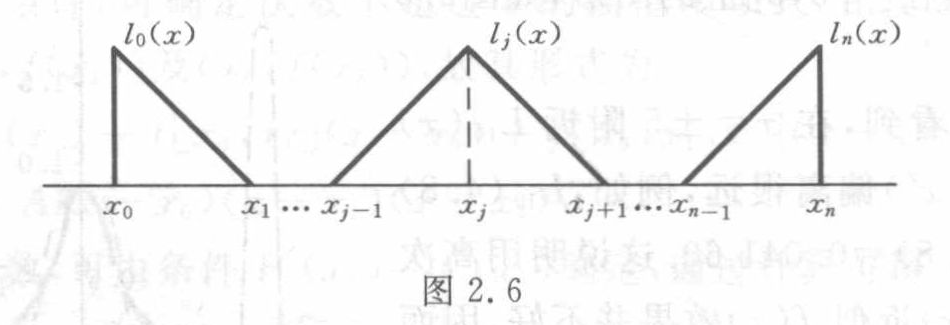
\includegraphics[width=0.85\linewidth,height=\textheight,keepaspectratio,alt={图 2.6（原图裁切）}]{../assets/ch02b/figure-2-6.png}

\begin{quote}
图 2.6（原图）：分段线性插值基函数的局部非零形状。左端 \(l_0(x)\) 在 \(x_0\) 达到峰值并线性降到 \(x_1\)；内部 \(l_j(x)\) 在 \(x_{j-1},x_{j+1}\) 为零，在 \(x_j\) 达到峰值；右端 \(l_n(x)\) 从 \(x_{n-1}\) 线性升到 \(x_n\)。全部原图标签为 \(l_0(x),\allowbreak l_j(x),\allowbreak l_n(x),\allowbreak x_0,\allowbreak x_1,\allowbreak \cdots,\allowbreak x_{j-1},\allowbreak x_j,\allowbreak x_{j+1},\allowbreak \cdots,\allowbreak x_{n-1},\allowbreak x_n\)；峰值未标数字。
\end{quote}

现在证明 \(\lim_{h\to0}I_h(x)=f(x)\)。考虑

\[\begin{aligned}
|f(x)-I_h(x)|&\leqslant l_k(x)|f(x)-f_k|+l_{k+1}(x)|f(x)-f_{k+1}|\\
&\leqslant[l_k(x)+l_{k+1}(x)]\omega(h_k)\\
&=\omega(h_k)\leqslant\omega(h),
\end{aligned}\tag{2.7.4}\]

这里 \(\omega(h)\) 是函数 \(f(x)\) 在区间 \([a,b]\) 上的\textbf{连续模}，即对于任意两点 \(x',x''\in[a,b]\)，只要 \(|x'-x''|\leqslant h\)，就有

\[|f(x')-f(x'')|\leqslant\omega(h),\]

称 \(\omega(h)\) 为 \(f(x)\) 在 \([a,b]\) 上的连续模，当 \(f(x)\in C[a,b]\) 时，就有 \(\lim_{h\to0}\omega(h)=0\)。

由前式可知，当 \(x\in[a,b]\) 时有 \(\max_{a\leqslant x\leqslant b}|f(x)-I_h(x)|\leqslant\omega(h)\)，因此，只要 \(f(x)\in C[a,b]\)，就有 \(\lim_{h\to0}I_h(x)=f(x)\) 在 \([a,b]\) 上一致成立，故 \(I_h(x)\) 在 \([a,b]\) 上一致收敛到 \(f(x)\)。

\subsection{本节覆盖原页的校注记录}\label{ux672cux8282ux8986ux76d6ux539fux9875ux7684ux6821ux6ce8ux8bb0ux5f55}

下列记录按原页关联，含同页相邻小节的校注；计算时同时读取上文校注和完整原页。

\begin{itemize}
\tightlist
\item
  \texttt{ch02b-E001}：原书 PDF 页 46
\end{itemize}

\end{document}
